\documentclass[a4paper,12pt]{article}
\usepackage{graphicx}
\usepackage[a4paper,margin=1in]{geometry}
\usepackage{titlesec}
\usepackage{hyperref}
\usepackage{amsmath}    % For math environments and symbols
\usepackage{amssymb}    % For \mathbb and other math symbols
\usepackage{amsfonts}   % Additional math fonts
\usepackage[backend=biber,style=numeric,sorting=none]{biblatex}
\usepackage{float}
\setlength{\abovecaptionskip}{-2pt}  
\setlength{\belowcaptionskip}{1pt}
\usepackage{subcaption}

\addbibresource{references.bib} % Add references.bib with the appropriate entries

% Title format
\titleformat{\section}{\large\bfseries}{\thesection}{1em}{}

% Title settings
\title{
    \includegraphics[scale=0.4]{Cam_logo_bw.png}\\
    \vspace{0.5cm}
    S2 Advanced Statistical Methods for Data Science - Coursework Assignment
}
\author{Raunaq Rai (rsr45@cam.ac.uk)\\
    Data Intensive Science, Department of Physics, University of Cambridge
}
\date{04 April, 2025 \\ \vspace{0.2cm} {\small Word Count: XXX}}

\begin{document}

\maketitle

\section*{Introduction}

The Antikythera Mechanism is one of the most remarkable technological discoveries from the ancient world. Found in 1901 (by accident) in a shipwreck near the Greek island of Antikythera, the device dates back to between 140 and 60 BCE (perhaps another opportunity for bayesian inference). What makes it so extraordinary is its system of bronze gears, which could be manually turned to display a wide range of astronomical phenomena. Housed in a wooden box, the mechanism likely showed the positions of the Sun and Moon, lunar phases, eclipse predictions, and even events tied to the ancient Greek calendar such as the Olympic Games \cite{Seiradakis2018}.

Thanks to modern imaging techniques like X-ray tomography, researchers have been able to reconstruct parts of the mechanism and get a clearer picture of how it worked. One key component is the calendar ring — a circular disk punctured with holes arranged around its edge. Only part of this ring survives, but it provides a fascinating clue to the type of calendar the device may have used. While it was once thought to represent a 365-day solar calendar, new analysis suggests it may instead follow a 354-day lunar cycle \cite{Budiselic2021}.

In this project, I tackle a Bayesian inference problem related to this calendar ring: how many holes did the full ring originally contain? Using the known positions of 81 holes across eight broken and misaligned fragments, I apply Hamiltonian Monte Carlo to estimate the total number of holes. Two different models are used to account for uncertainties in the hole positions: one assuming isotropic Gaussian error, and another that separates radial and tangential uncertainties \cite{Woan2024}. By comparing the results from both models, I aim to determine which best fits the data and what this can tell us about how the mechanism was designed and about the way time was measured in the ancient world.

\begin{figure}[t!]
    \centering
    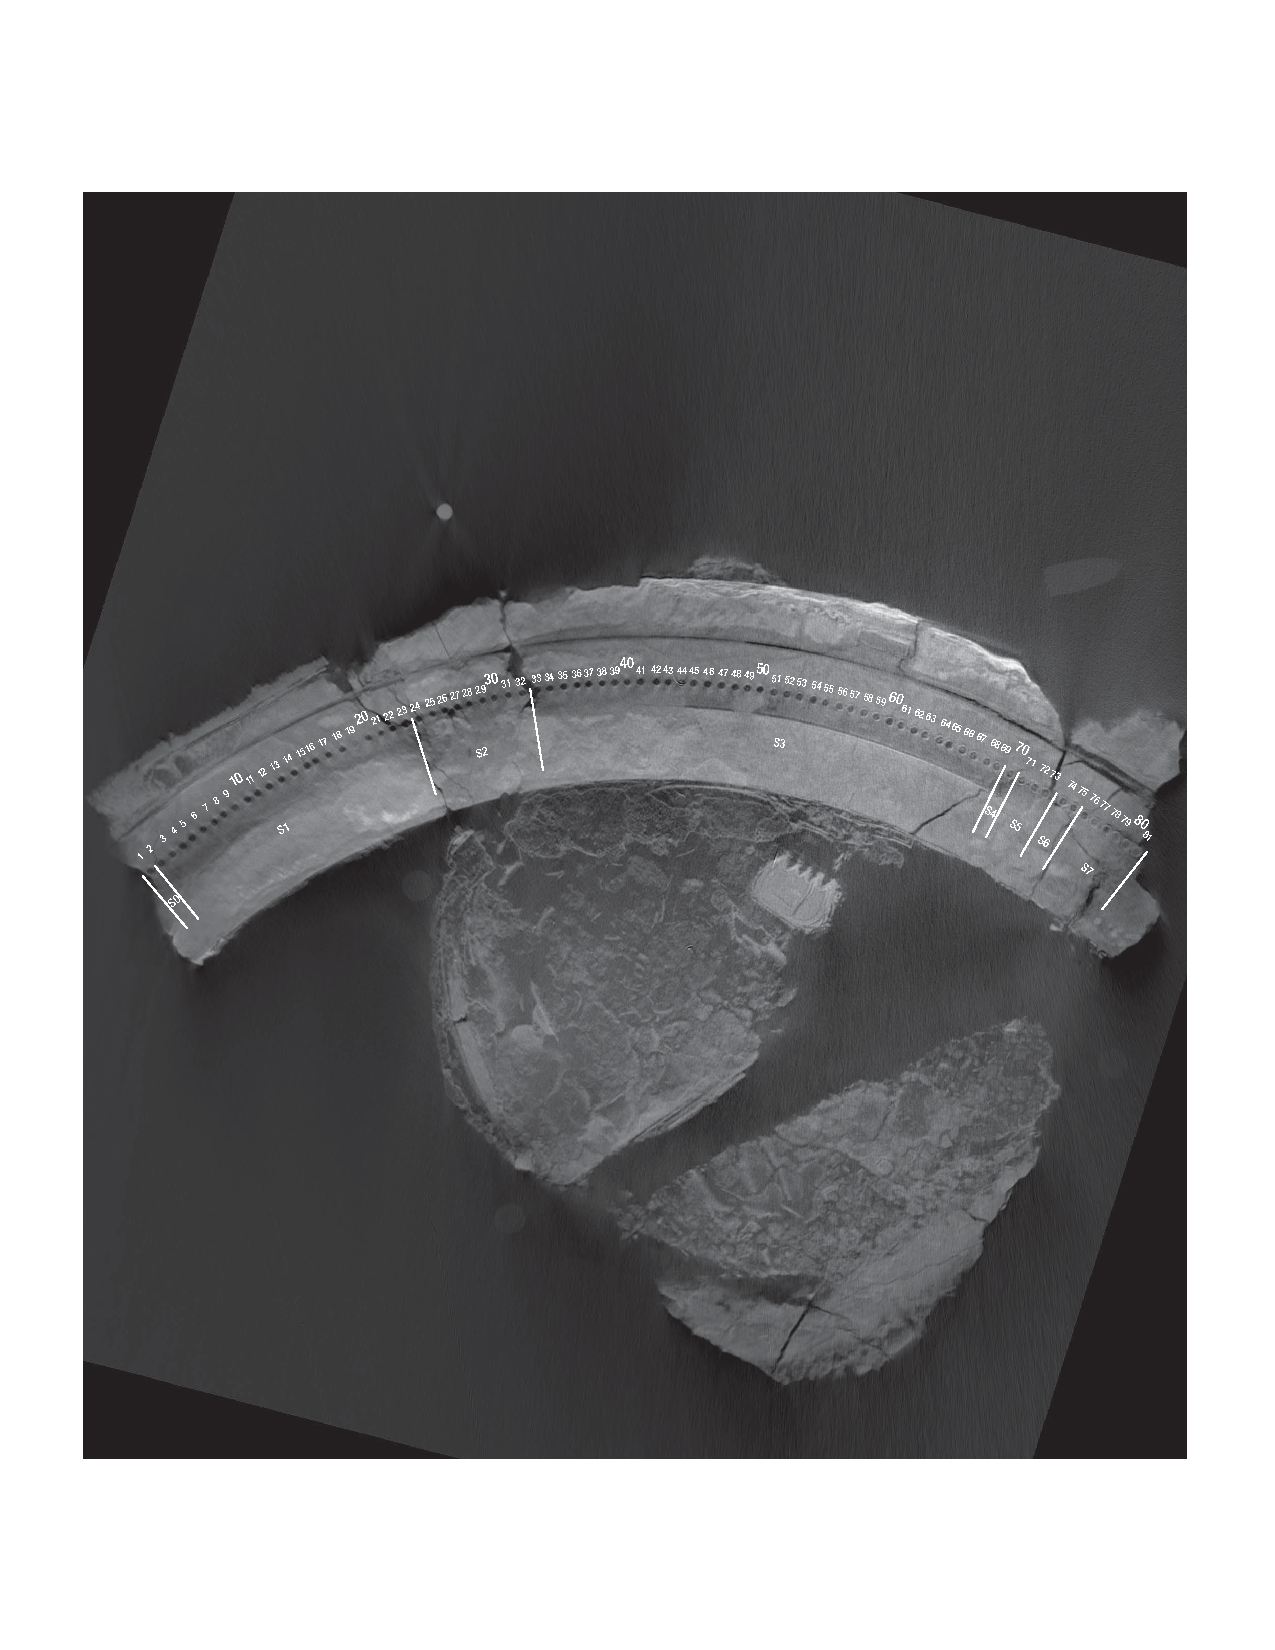
\includegraphics[width=0.8\textwidth]{Xray_antikythera.pdf}
    \vspace{0.5cm}
    \caption{X-ray image of the surviving fragments of the Antikythera Mechanism.}
    \label{fig:xray}
\end{figure}

\section{Measured Hole Locations $d_i \in \mathbb{R}^2$ in the $x$-$y$ Plane}

The data used in this analysis was obtained from the public dataset provided by Thoeni, Budiselic, and Ramsey~\cite{Thoeni2019}. The dataset contains the $x$ and $y$ coordinates of 81 holes in the surviving fragments of the calendar ring. These holes are distributed across eight fragments, each of which is colour-coded in Figure~\ref{fig:parta}. This visualisation provides an initial sense of the ring's geometry and the extent of its misalignment.

\begin{figure}[t!]
    \centering
    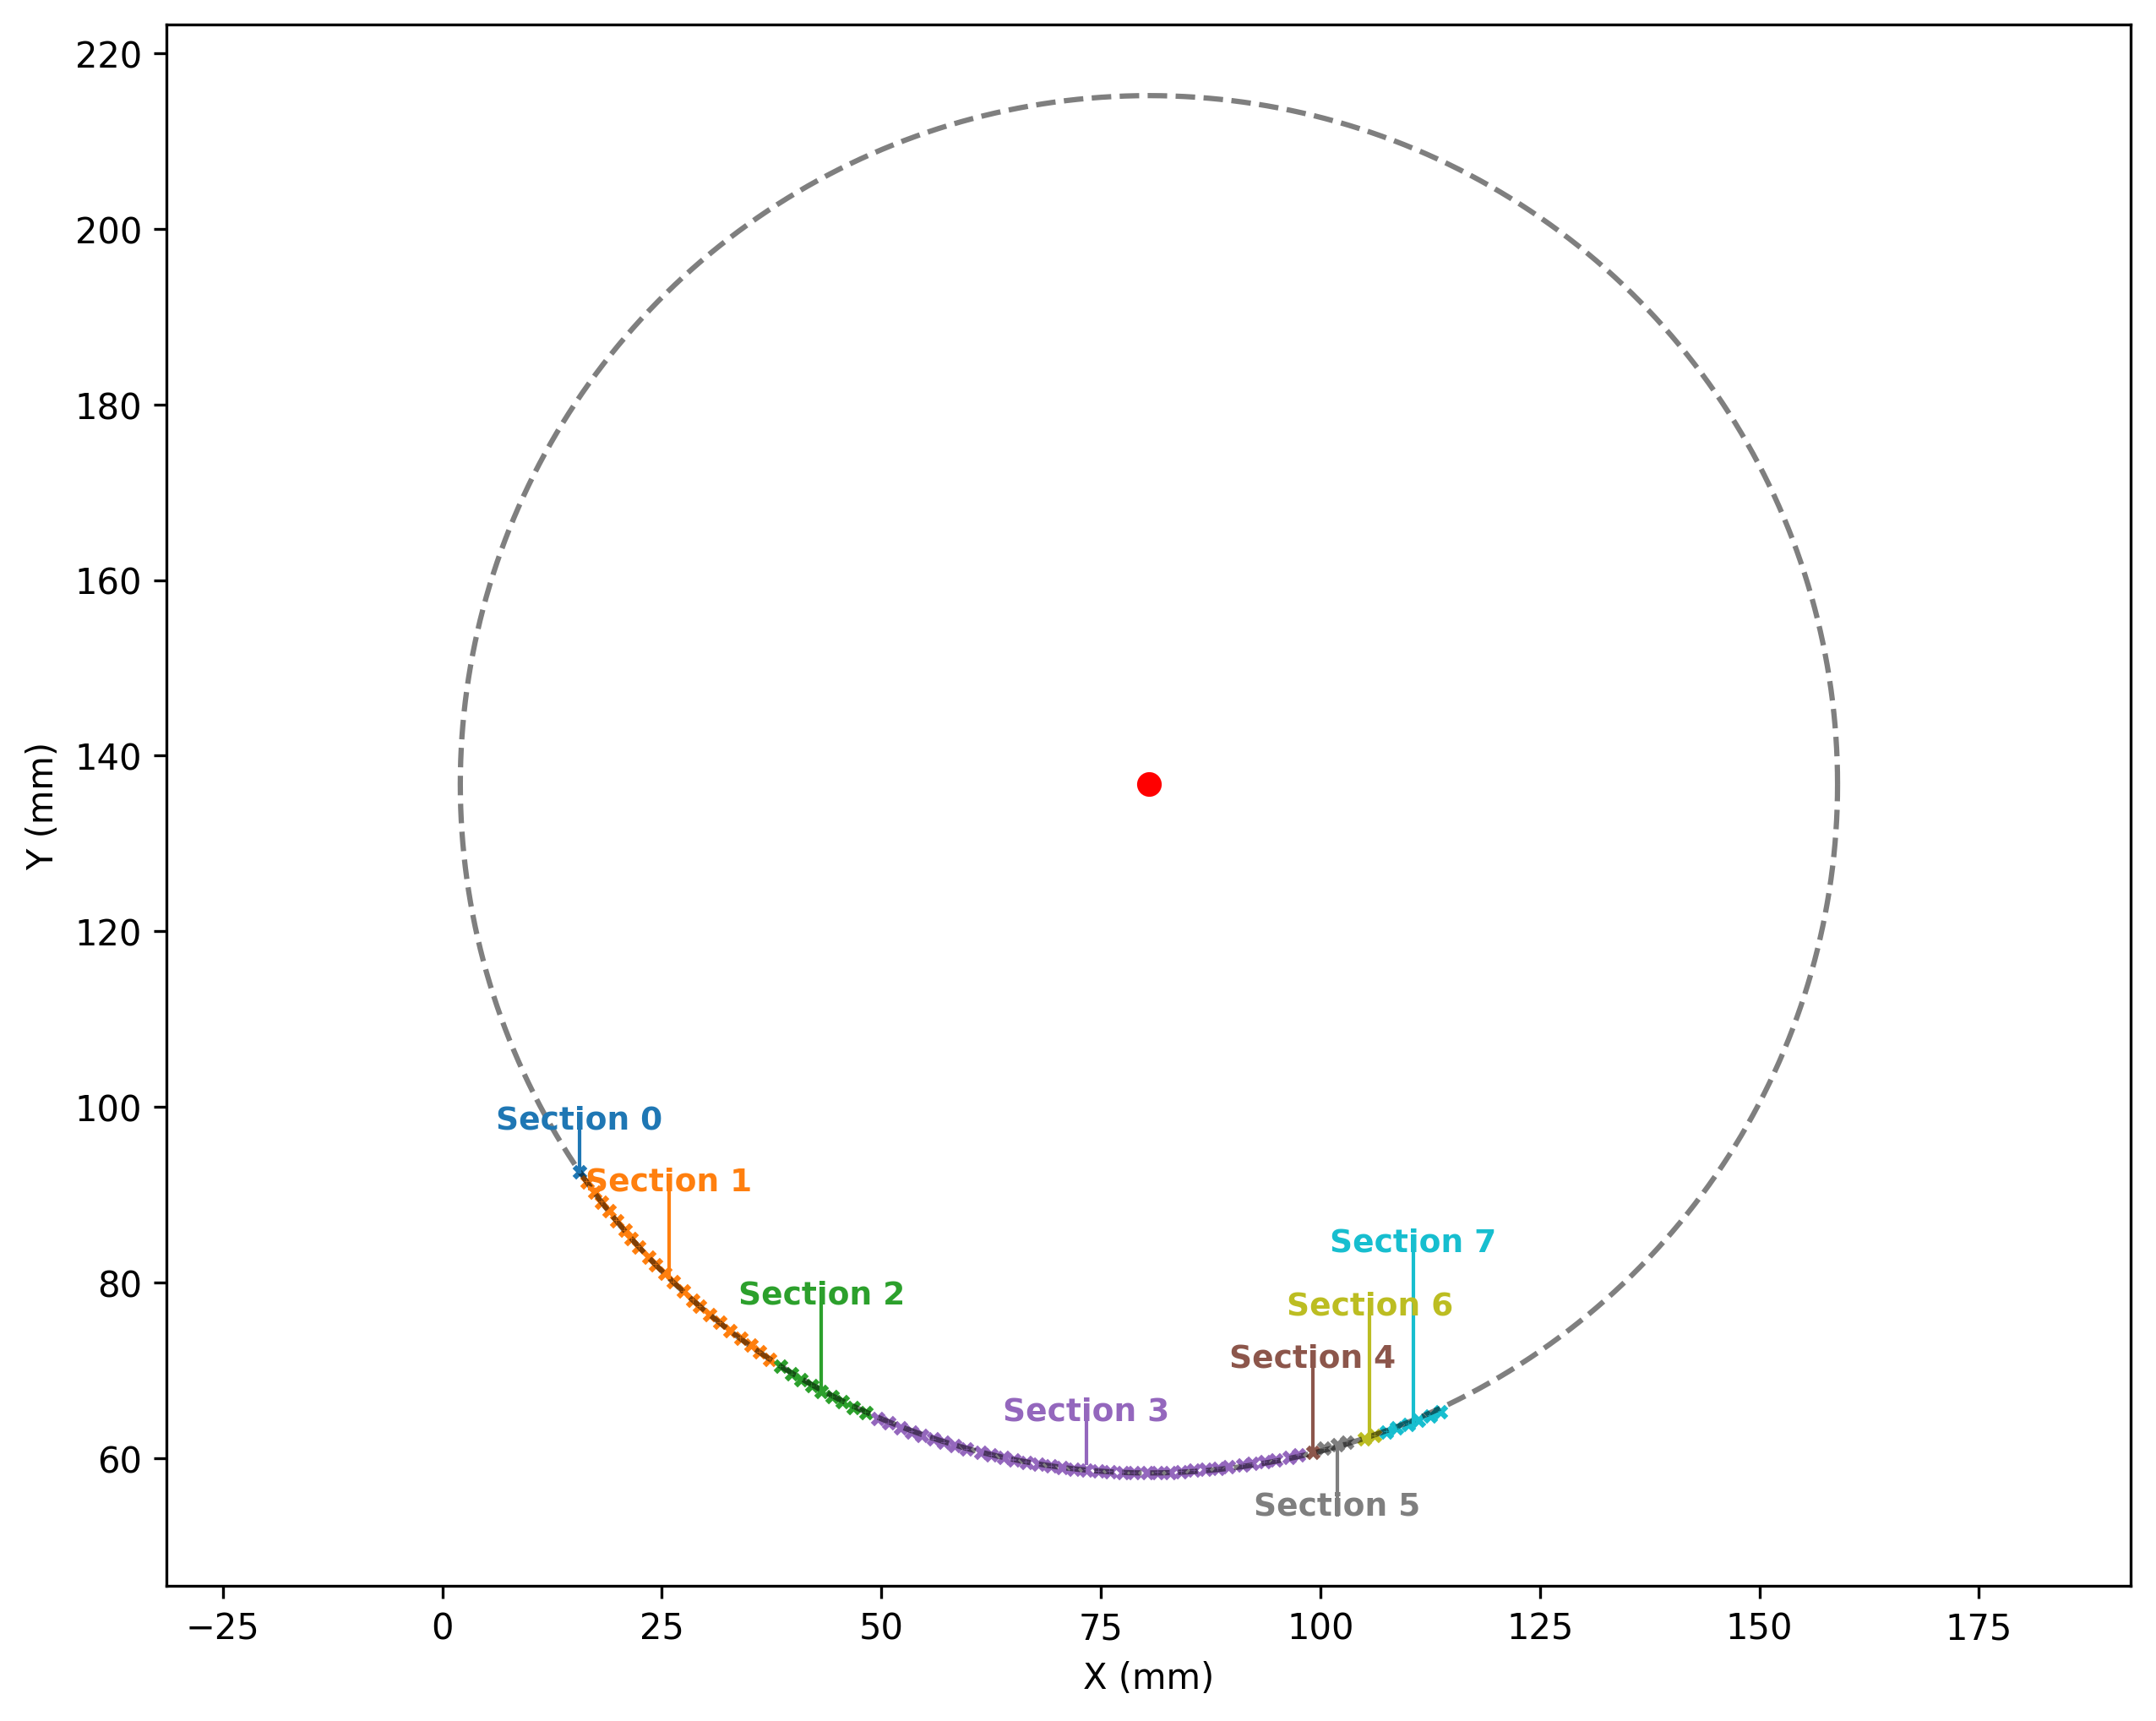
\includegraphics[width=0.85\textwidth]{part_a.png}
    \caption{Measured hole locations $d_i \in \mathbb{R}^2$ in the $x$-$y$ plane, colour-coded by fractured ring segment. The dashed circle shows the estimated full ring, fitted to the data using a non-linear least-squares method. Section labels are placed to minimise overlap and connected to the median point of each segment.}
    \label{fig:parta}
\end{figure}

\section{Hole Location model}

Following the model described in Section 2 of Woan and Bayley~\cite{Woan2024}, we assume that the original calendar ring contained $N$ holes, evenly spaced around a circle of radius $r$. The full ring no longer survives, and the measured hole locations come from $s = 8$ fragmented sections. Each fragment is slightly misaligned due to relative translations and in-plane rotations.

The Cartesian coordinates of the $i$-th hole in a given section can be modelled as:
\begin{equation}
    \vec{m}_i = 
    \begin{pmatrix}
        x_i \\
        y_i
    \end{pmatrix}
    =
    \begin{pmatrix}
        r \cos\left( \frac{2\pi(i-1)}{N} + \alpha_j \right) + x_{0j} \\
        r \sin\left( \frac{2\pi(i-1)}{N} + \alpha_j \right) + y_{0j}
    \end{pmatrix},
    \label{eq:model}
\end{equation}
where $(x_{0j}, y_{0j})$ is the translation of section $j$, and $\alpha_j$ is its relative angular offset. The model assumes all fragments lie in the same $x$-$y$ plane and are internally undistorted.

\section{Likelihood Model}

To assess how well the model predicts observed hole locations, we use a Gaussian likelihood for each measured hole $\vec{d}_i = (x_i, y_i)$, under the assumption that errors are independent across holes. The likelihood for a single hole is given by:

\begin{equation}
    p(\vec{d}_i \mid \vec{m}_i, \Sigma) = \frac{1}{2\pi \sqrt{|\Sigma|}} \exp\left( -\frac{1}{2} (\vec{d}_i - \vec{m}_i)^\top \Sigma^{-1} (\vec{d}_i - \vec{m}_i) \right),
\end{equation}

where $\vec{m}_i = (x_i^{\text{model}}, y_i^{\text{model}})$ is the model prediction for hole $i$ and $\Sigma$ is the $2 \times 2$ covariance matrix describing measurement uncertainty. The total log-likelihood over all holes is then:

\begin{equation}
    \log \mathcal{L}(\theta) = -\frac{1}{2} \sum_{i=1}^{N_\text{holes}} \left[ (\vec{d}_i - \vec{m}_i)^\top \Sigma^{-1} (\vec{d}_i - \vec{m}_i) + \log(2\pi |\Sigma|) \right].
\end{equation}

\paragraph{Isotropic model.}  
In the isotropic case, we assume errors are equal in all directions:
\begin{equation}
    \Sigma = \sigma^2 I, \quad \Sigma^{-1} = \frac{1}{\sigma^2} I, \quad |\Sigma| = \sigma^4.
\end{equation}

\paragraph{Anisotropic (radial-tangential) model.}  
In this model, uncertainties are decomposed into radial and tangential directions. For a predicted hole location at angle $\phi_i$, we define the local coordinate frame as:

\begin{align}
    \text{Radial unit vector:} & \quad \hat{r}_i = \begin{pmatrix} \cos\phi_i \\ \sin\phi_i \end{pmatrix}, \\
    \text{Tangential unit vector:} & \quad \hat{t}_i = \begin{pmatrix} -\sin\phi_i \\ \cos\phi_i \end{pmatrix}.
\end{align}

The displacement vector $\vec{\delta}_i = \vec{d}_i - \vec{m}_i$ is then projected as:

\begin{align}
    \delta_{r,i} &= \hat{r}_i^\top \vec{\delta}_i = (x_i - x_i^{\text{model}})\cos\phi_i + (y_i - y_i^{\text{model}})\sin\phi_i, \\
    \delta_{t,i} &= \hat{t}_i^\top \vec{\delta}_i = -(x_i - x_i^{\text{model}})\sin\phi_i + (y_i - y_i^{\text{model}})\cos\phi_i.
\end{align}

The radial-tangential errors are then treated as a 2D Gaussian with diagonal covariance:

\begin{equation}
    \Sigma_{\text{rt}} = \begin{pmatrix} \sigma_r^2 & 0 \\ 0 & \sigma_t^2 \end{pmatrix}, \quad
    \Sigma_{\text{rt}}^{-1} = \begin{pmatrix} 1/\sigma_r^2 & 0 \\ 0 & 1/\sigma_t^2 \end{pmatrix}, \quad
    |\Sigma_{\text{rt}}| = \sigma_r^2 \sigma_t^2.
\end{equation}

The Mahalanobis distance in this frame becomes:

\begin{equation}
    D^2_i = \begin{pmatrix} \delta_{r,i} \\ \delta_{t,i} \end{pmatrix}^\top
            \Sigma_{\text{rt}}^{-1}
            \begin{pmatrix} \delta_{r,i} \\ \delta_{t,i} \end{pmatrix}
          = \frac{\delta_{r,i}^2}{\sigma_r^2} + \frac{\delta_{t,i}^2}{\sigma_t^2}.
\end{equation}

Both the isotropic and anisotropic log-likelihoods were implemented in NumPy and JAX. The JAX version is compatible with automatic differentiation, Numpyro and Hamiltonian Monte Carlo. It was validated against the NumPy implementation and used in all posterior sampling analyses.




\printbibliography{}

\end{document}
